\section{$X_{i}$を等確率で選び,その中から$x$が一様に選ばれる場合}

この設定は,はじめに$N$個の集合$X$から1つの$X_{i}$選択し,点$x$はそれぞれの $X_{i}$について$\Omega = [0,1]$に一様に分布しているとする。このとき,$X_{i}$の数$N$が変化しても,$x$についての選び方は同じであるから,$x$の作るネットワークだけでは,本来考えたい$N$との間の関係は見ることができない。しかしながら,選ばれた点のネットワークに関する性質を調べるには良い練習となる。

$X_{i}$から$k$番目に点が選ばれ,その後時刻$k+1$に$X_{j}$から点が選ばれる確率は,$X_{i}$の数$N$として
\[p_{i}(k,j) = p(N) = \frac{1}{N}\]
のように,直前の履歴に依存せず,等確率である場合を考えている。

このとき,$x$は$[0,1]$の間の値を一様な確率で取るとしていたので,そうして得られた確率変数$x$に関して,
確率密度関数$f(x)$は
\[f(x) = 1\ \ \ (0\le x \le 1)\ \ \ \text{otherwise}\ \ 0\]
であり,累積分布関数$F(x)$は
\[F(x) = x\ \ \ (0\le x \le 1)\]
である。

時間発展によって点が選ばれていくごとに,その点と距離$r$より近い位置にある点との間にすべてエッジを張っていくことにする。すなわち,この問題はある閾値$r(0<r\le1)$を定めた時に,時刻$k$で選ばれた点$x_{k}$を中心とする領域$[x^{k}-r, x^{k}+r]$の中に入るそれまでに出た点の数はいくつか,という問題に帰着される。

すなわち図\ref{fig:f2}のような状況を考えていることになる。
\begin{figure}[H]
    \begin{center}
        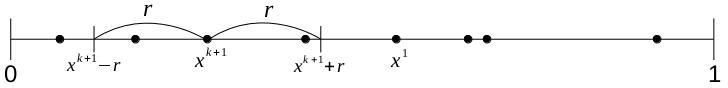
\includegraphics[width=10cm]{../simple1/simple001_1.jpg}
        \caption{$[0,1]$の数直線上で閾値$r$で定められる領域}
        \label{fig:f2}
    \end{center}
\end{figure}

一様な確率で$[0,1]$の間の数が選ばれるとき,その確率変数が$[\max(0,x-r), \min(x+r,1)]$の範囲に入っている確率は,確率密度関数を用いて,
\begin{align}
p(\max(0, x-r), \min(x+r, 1)) &= \int ^{\min(x+r,1)}_{\max(0, x-r)} 1 dx \nonumber \\
&= \left[ x\right]^{\min(x+r,1)}_{\max(0, x-r)}
\end{align}
よって
\begin{eqnarray}
p(x,r)= \left\{ \begin{array}{ll}x+r & 0\le x< \min(r,1-r) \nonumber \\
p(r) = \min(2r, 1) & \min(r, 1-r)\le x \le \max(1-r, r) \nonumber \\
1 - x+r & \max(1-r, r) < x \le 1
\end{array}\right.
\end{eqnarray}
を得る。

これはグラフにすると,図\ref{fig:f3}のようになる。
\begin{figure}[H]
    \begin{center}
        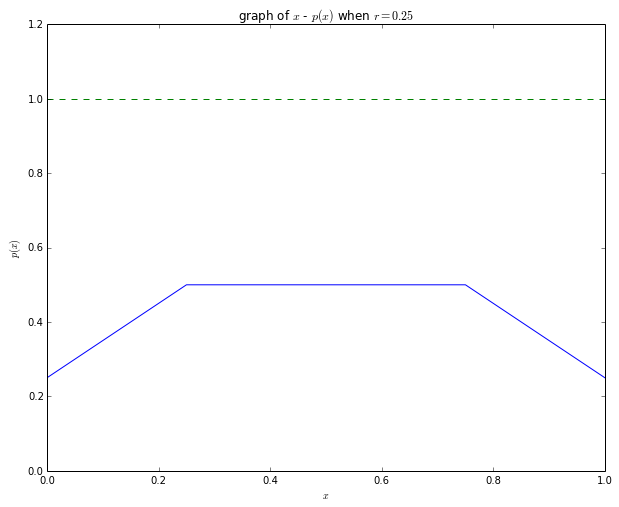
\includegraphics[width=10cm]{../img/fig3.png}
        \caption{$r=0.25$のとき,それぞれの位置$x$において他の点を1つ見出す確率$p(x)$}
        \label{fig:f3}
    \end{center}
\end{figure}

$k+1$番目に点$x_{k+1}$が選ばれたとき,$k$番目までに選ばれた点のうち$y$個の点が領域$[\max(0,x-r), \min(x+r,1)]$の中に存在する確率は,
\begin{eqnarray}
_{k}C_{y}p(r)^{y}p(r)^{k-y}
\label{eq:e1}
\end{eqnarray}
で表せる。ここで注意すべき点は,$p(x_{k}, r)$は$x_{k}$によって変わるものであったから,$x$に対して期待値を取ったものを考えなければならないことである。$p(r)$はそのようにして得られた期待値であることを意味している。

$p(r)$を求めると,
$0<r\le0.5$のとき
\begin{align}p(r) = E(p(x, r)) &= \int^{r}_{0}x+r\mathrm{d}x + \int^{1-r}_{r}2r \mathrm{d}x + \int^{1}_{1-r} 1-x+r \mathrm{d}x\nonumber \\
&= \left[\frac{x^{2}}{2} + rx \right]^{r}_{0} + \left[ 2rx\right]^{1-r}_{r}+ \left[ x-\frac{x^{2}}{2} + rx\right]^{1}_{1-r}\nonumber \\
&= -r^{2} + 2r \end{align}
$0.5<r\le1$のときも同様にして
\[p(r) = E(p(x,r)) = -r^{2} + 2r\]
である。

また,式(\ref{eq:e1})は
\[P[X=y] =\ _{k}C_{y}p(r)^{y}(1-p(r))^{k-y}\]
のように書けば明らかなように,確率変数$X$に対するパラメータ$k,p$の二項分布$B(k,p)$を表している。

この時,確率変数$X$に対する期待値と分散は,
\[E(X) = kp(r)\]
\[V(X) = kp(r)(1-p(r))\]
である。

時刻$k$が大きい時,具体的には
\[kp(r) > 5,\]
\[kp(r)(1-p(r)) > 5\]
をみたす$k$のとき,二項分布は正規分布に近似できるので,期待値は中央値とほぼ等しくなる。すなわち,$y=kp(r)$より多くの点を見出す確率$P[X\le y]$は,どんな時刻$k$においても$1/2$となる。

すなわち,時刻の依存性はないため,$x_{k+1}$のまわりの領域に$y$個以上の他の点が存在する場合を1,存在しない場合を0とすれば,これらの起こる確率は,それぞれ$1/2$であり,$k$回目に$y$個以上のエッジが張られる確率は,$p=1/2$の幾何分布に従う:
\[P[X=k] = \left( \frac{1}{2} \right)^{k}\]
このときの期待値と分散は
\[E(X) = \frac{1}{p} = 2\]
\[V(X) = \frac{1-p}{p^{2}} = 2\]

すなわち,これまでのような場合を考えたとすると,平均として2回で$y$個以上のエッジが張られ,ほとんどの試行は$1\sim3$回でその値に到達することが分かる。しかし,これは先程述べたような二項分布の正規分布への近似ができない領域であることに注意が必要である。
